%\chapter*{Première Partie : titre}
%\setcounter{chapter}{1}  % Đặt lại số chương thành 1
% đẩy phần JO lên đầu

\chapter{Sénat et Projet de Tables du Sénat}

\section{Sénat et Archives du Sénat}

\subsection{Sénat et ses missions}
Le Sénat est l'une des deux assemblées qui représente la France, avec l'Assemblée nationale. Ce système à deux chambres s'appelle le « bicamérisme ». Les deux chambres partagent des rôles similaires : elles discutent et modifient les lois, se penchent sur des sujets nationaux importants, et surveillent le travail du gouvernement. Toutefois, contrairement à l'Assemblée nationale, le Sénat protège aussi les intérêts des régions, départements et communes, qu'on appelle les « collectivités territoriales ». Si les deux chambres ne sont pas d'accord sur une loi, c'est l'Assemblée nationale qui a le dernier mot. \footcite{Essentiel}

Il est composé de 345 Sénateur, qui représentent les citoyens, débattent, rédigent des lois et vérifient les actions du gouvernement. Ils étudient les projets de loi proposés par ce dernier et peuvent également soumettre leurs propres propositions. De plus, ils examinent les politiques publiques et peuvent créer des groupes temporaires pour analyser des questions spécifiques et proposer des réformes. Les propositions de loi des deux Assemblées ainsi que leur parcours parlementaire sont référencées sur le site du Sénat.\footcite{indexpropositionsdeloi} Le Sénat assure également la stabilité des institutions, car il ne peut pas être dissous, contrairement à l'Assemblée nationale. Enfin, en cas de vacance ou d'empêchement du Président de la République, c'est le Président du Sénat qui assure l'intérim.\footcite{Essentiel}

\subsection{Fonction de la séance publique}
"Le Sénat ne siège pas uniquement en séance plénière : il comporte également des commissions composées d’un nombre restreint de sénateurs. Tous les sénateurs, à l’exception du Président du Sénat, font partie d’une commission permanente et d’une seule.\footcite{Recueildefichesdusenat}

Le point clé du fonctionnement et de l’influence des commissions permanentes réside dans le mode de désignation de leurs membres. À cet effet, après chaque renouvellement triennal, les groupes politiques établissent, par accord mutuel et au prorata de leurs effectifs, une liste de candidats qui est affichée puis – normalement – ratifiée par le Sénat.\footcite{Recueildefichesdusenat}

Les commissions permanentes jouent un rôle essentiel dans la préparation du travail législatif, dans le contrôle du Gouvernement et dans l’information des sénateurs.

Actuellement, les 8 commissions permanentes du Sénat sont les suivantes :
- Commission de la culture, de l’éducation, de la communication et du sport (49 membres) ;
- Commission des Affaires économiques,(50 membres) ;
- Commission des Affaires étrangères, de la Défense et des Forces armées, pour le contrôle de l’exécution de la loi de programmation et du budget de la défense, le débat et le vote sur l’intervention des forces armées à l’étranger ou les relations interparlementaires (48 membres) ;\footcite{fichecommissionaffairesetrangeres}
- Commission des Finances, pour le Contrôle du budget et des Comptes économiques de la Nation (49 membres) ;
- Commission des lois constitutionnelles, de législation, du suffrage universel, du Règlement et d'administration générale (48 membres) ;
- Commission des affaires sociales (51 membres) ;
- Commission de l'aménagement du territoire et de développement durable (49 membres) ;
- Commission des affaires européennes, pour le contrôle et le suivi de l'action européenne de l'exécutif, le contrôle et suivi des politiques et institutions de l'Union européenne, ainsi que la coopération avec les autres parlements de l'Union européenne (40 membres) ;\footcite{lescommissionspermanentes}

Dans la séance, les sénateurs discutent des grandes idées de chaque texte de loi, puis l'examinent en détail, article par article. Ils peuvent apporter des modifications en proposant des amendements. Pendant des séances spéciales, les ministres sont tenus de répondre aux questions des sénateurs.

Avant d'être débattu en séance publique, chaque texte est d'abord étudié par une commission spécialisée sur le sujet. Dans cette commission, les sénateurs choisissent un rapporteur pour chaque texte. Ce rapporteur analyse le texte et fait des recommandations, comme supprimer, ajouter ou modifier un article, ce sont les amendements\footcite{lescommissionspermanentes}. Les commissions organisent aussi régulièrement des auditions avec des ministres, des responsables publics, des ambassadeurs, des ministres étrangers, des commissaires européens, ainsi que des représentants de la société civile ou du secteur privé. En outre, la commission des affaires européennes a pour mission de fournir des informations et de surveiller les activités européennes.

\section{Archives du Sénat et fonction des Archives du Sénat}

\subsection{Présentation des archives}

Conformément à l'article 20 du Règlement intérieur du Sénat, la Direction de la Bibliothèque et des Archives a pour mission de collecter, classer, conserver, et rendre accessibles les archives du Sénat. Elle est également responsable de la rédaction et de l'impression des tables annuelles des comptes rendus des séances, ainsi que de la création des dossiers biographiques des sénateurs et de la rédaction du *Dictionnaire des parlementaires français*, notamment pour les notices concernant les sénateurs. Ces tâches sont accomplies par la division des Archives, qui met en œuvre ces missions au service des chercheurs. \footcite{GuideduLecteur}

La division est chargée de l'élaboration des tables nominatives et thématiques des travaux du Sénat. Cela inclut la collecte de documents provenant des différentes directions, quel qu'en soit le support (papier, vidéo, numérique, photographique, etc.). La typologie, la durée de conservation et les règles de gestion de ces documents sont définies dans un tableau de gestion. Les documents destinés à être conservés définitivement doivent être transférés à la division à la fin de leur durée d'utilité administrative. Ils sont ensuite répertoriés dans un bordereau de versement, co-signé par la direction concernée et la Direction de la Bibliothèque et des Archives, puis intégrés dans un logiciel de gestion d'archives pour un accès rapide et facile. \footcite{GuideduLecteur}

Une fois sous la garde de la division, les archives du Sénat sont conservées dans des matériaux neutres et stockées dans des locaux spécialement dédiés pour en assurer la préservation à long terme. La division surveille régulièrement leur état et procède aux restaurations nécessaires. Par ailleurs, une partie des documents, comme les enregistrements audio et audiovisuels des séances publiques, a été numérisée pour en garantir la pérennité et en faciliter l'accès. \footcite{GuideduLecteur}

Les archives du Sénat, qui sont d’une grande richesse, incluent notamment des dossiers législatifs et des procès-verbaux des commissions depuis la IIIe République, des archives de la Trésorerie et de la Questure depuis le Premier Empire, ainsi que des procès devant la Haute Cour de Justice et des archives du Sénat de la Communauté. En 1848, après la disparition de la seconde chambre, une partie importante des archives du Sénat conservateur et de la Chambre des pairs fut transférée aux Archives nationales. En 1921, en raison du manque de place, certaines archives du Second Empire furent également versées. Aujourd'hui, presque toutes les archives sous la responsabilité du Sénat sont inventoriées, et une cinquantaine d'instruments de recherche permettent d’effectuer des recherches thématiques et nominatives.\footcite{GuideduLecteur}

Enfin, la division est également responsable de la constitution des dossiers biographiques des sénateurs, ainsi que de la gestion des enregistrements audiovisuels des séances publiques et des principales manifestations organisées au Sénat. \footcite{GuideduLecteur}


\subsection{Tables des débats du Sénat}

\subsubsection{Journal officiel (JO)}

Les séances du Sénat sont publiques conformément à l'article 33 de la Constitution, et leurs comptes rendus intégraux sont publiés dans le \textit{Journal Officiel}. Depuis le 4 juin 1996, le Sénat met à disposition sur son site Internet la version électronique de ces comptes rendus, réalisée par la direction du compte rendu intégral du Sénat. Ces documents sont disponibles au format \textit{html} dans un délai de 24 à 36 heures après la séance, et publiés dans le \textit{Journal Officiel des débats} sous 7 à 15 jours. À partir du 2 mai 2005, une version \textit{pdf}, réplique exacte de la version papier, est également accessible dans les mêmes délais depuis la page dédiée aux séances du mois ou à chaque séance spécifique. Les débats du Congrès du Parlement, à compter de la séance du 28 février 2005, sont disponibles en ligne, tandis que les comptes rendus antérieurs peuvent être consultés sur le site de l'Assemblée nationale. Pour la période allant de décembre 1958 à mai 1996, le compte rendu intégral est disponible au format \textit{pdf} grâce à la numérisation du \textit{Journal Officiel}, incluant pour les années 1958 à 1982 les questions écrites des sénateurs. Les débats de 1916 et 1917, tenus en comité secret et publiés dans le \textit{Journal officiel des débats du Sénat} du 29 septembre 1968, sont reproduits d’après les comptes rendus des séances de septembre 1968. Par ailleurs, les débats du Conseil de la République, pour la période de décembre 1946 à juin 1958, y compris les questions écrites, sont également accessibles sous forme numérisée dans le \textit{Journal Officiel} au format \textit{pdf}. Enfin, les comptes rendus intégraux des débats du Sénat couvrant la période de 1876 à 1940 sont disponibles sur la page consacrée aux travaux du Sénat de la IIIe République. Pour obtenir un résumé non officiel des débats, il est possible de consulter le compte rendu analytique. \footcite{senat_comptes_rendus}

\begin{figure}[H]
    \centering
    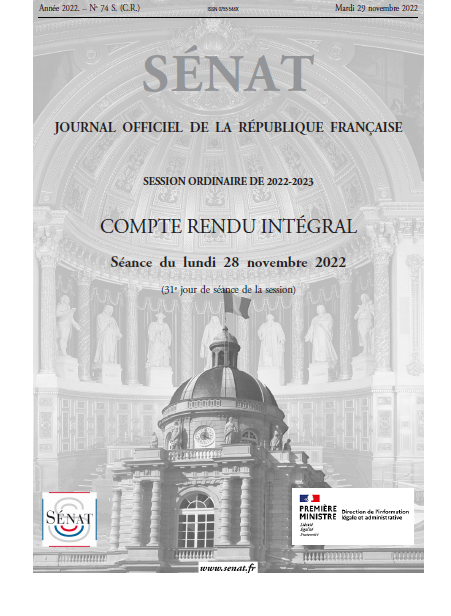
\includegraphics[width=0.6\textwidth]{images/JO.png}
    \caption{Image d'illustration d'un Journal officiel}
\end{figure}

\subsection{Historique et rôle des tables des matières dans les documents officiels du Sénat}

Les tables des matières sont des outils essentiels à la documentation des débats parlementaires du Sénat. Elles offrent une structure systématique qui permet de répertorier les interventions des sénateurs, les sujets débattus, ainsi que les actions législatives et non-législatives au sein des séances publiques et, depuis 2009, des commissions. Ces tables, produites annuellement, jouent un rôle crucial dans la transparence des travaux parlementaires en permettant aux chercheurs, aux journalistes et au grand public d'accéder facilement à l'information.\footcite{senat_tables_debats}

Le rôle des tables des matières a évolué au fil des décennies pour s'adapter aux besoins croissants de documentation et d'analyse. Elles ne se limitent plus à un simple index des interventions mais s'étendent à une classification détaillée des nominations, des dépôts législatifs, des questions, ainsi que des thèmes abordés lors des débats. Depuis avril 2009, elles incluent également les activités en commission, ce qui marque une étape importante dans l'exhaustivité des documents officiels.\footcite{senat_tables_debats}

\subsubsection{Présentation des différentes tables}

Les documents officiels du Sénat comprennent plusieurs types de tables des matières, chacune répondant à des besoins spécifiques en termes d'organisation et de consultation des données parlementaires :

\subsubsubsection{Table Nominative}

La Table nominative, ou Tome I, est un répertoire complet des activités individuelles des sénateurs pour une année donnée. Elle inclut un récapitulatif chronologique des nominations dans diverses commissions, des dépôts de propositions de loi, des interventions en séance publique, et, depuis 2009, des interventions en commission. Ce tome est un outil précieux pour l’analyse de la participation et des contributions des sénateurs. Il permet de retracer l’ensemble des actions parlementaires d’un sénateur sur une année et d’identifier ses domaines d’intervention.

\begin{figure}[H]
    \centering
    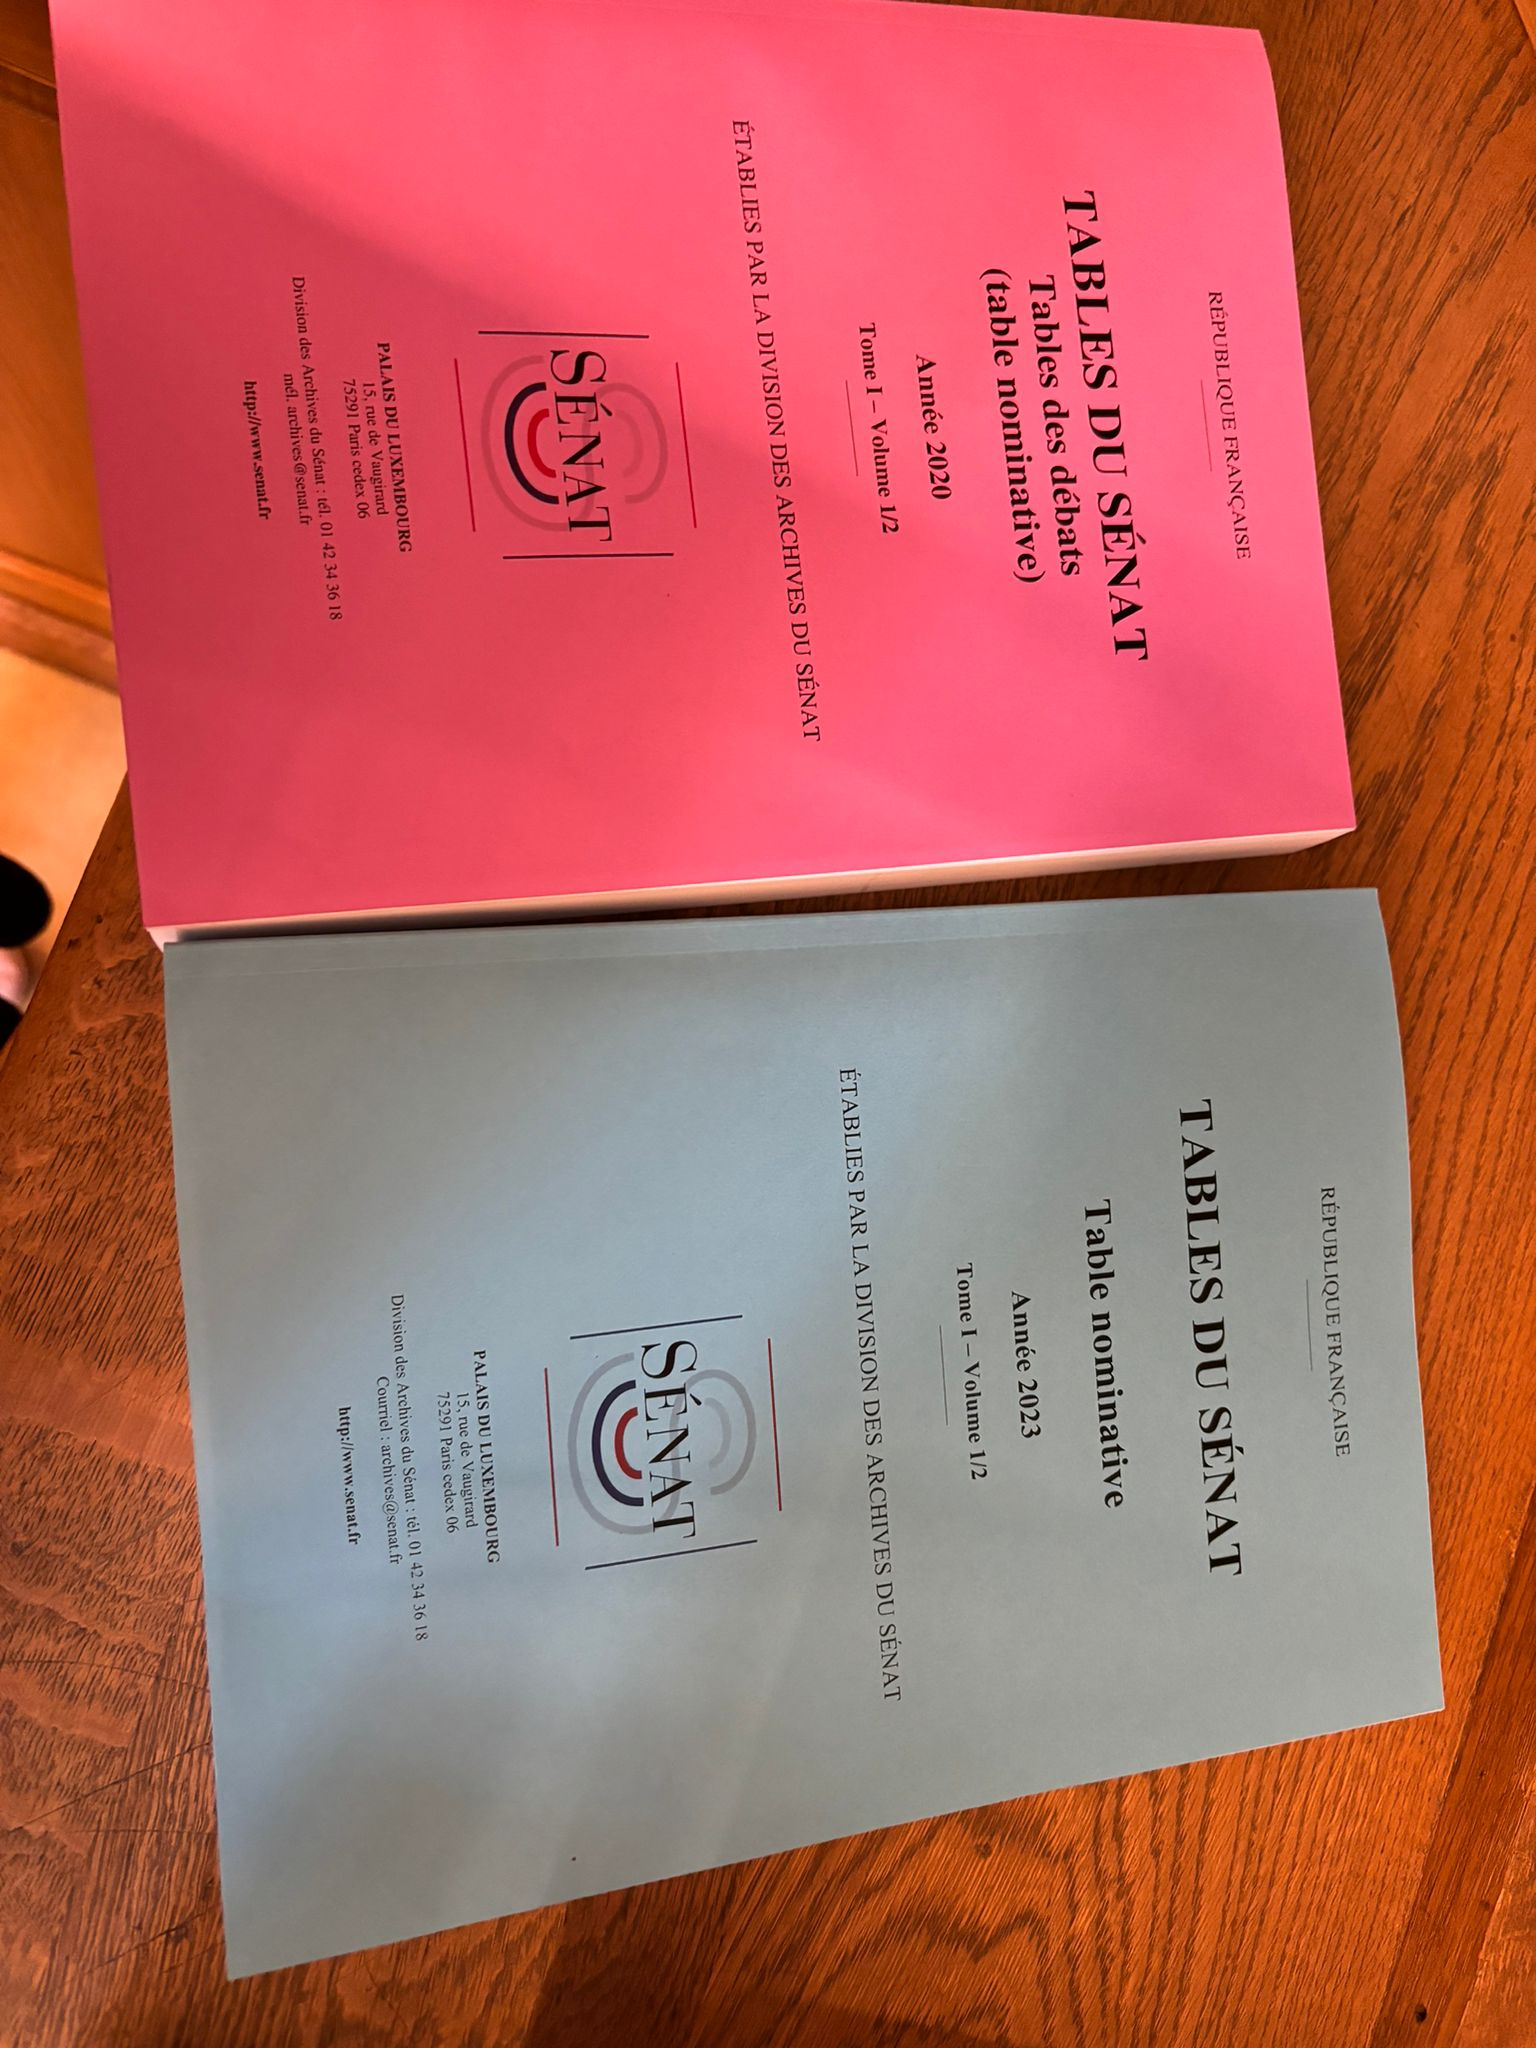
\includegraphics[angle=90, width=\textwidth]{images/tables nominatives.jpg}
    \caption{Photographie des tables nominatives du Sénat}
\end{figure}

Depuis 2017, deux innovations ont enrichi cette table : la mention des interventions, même lorsque la parole n'a pas été officiellement accordée, et la précision des sujets concernant les articles additionnels. Ces changements ont pour but de rendre compte de manière plus fidèle et complète des activités de chaque sénateur et sénatrice.

\subsubsubsection{Table Thématique}

La Table thématique, ou Tome II, organise les débats parlementaires selon les thèmes abordés au cours de l’année. Ce volume rassemble les propositions et projets de loi, les déclarations du gouvernement, les allocutions, et d’autres éléments comme les éloges funèbres et les motions de procédure. C'est un outil essentiel pour ceux qui cherchent à suivre l'évolution d'un sujet particulier sur plusieurs années, permettant de tracer les discussions législatives sur des thématiques spécifiques.

\begin{figure}[H]
    \centering
    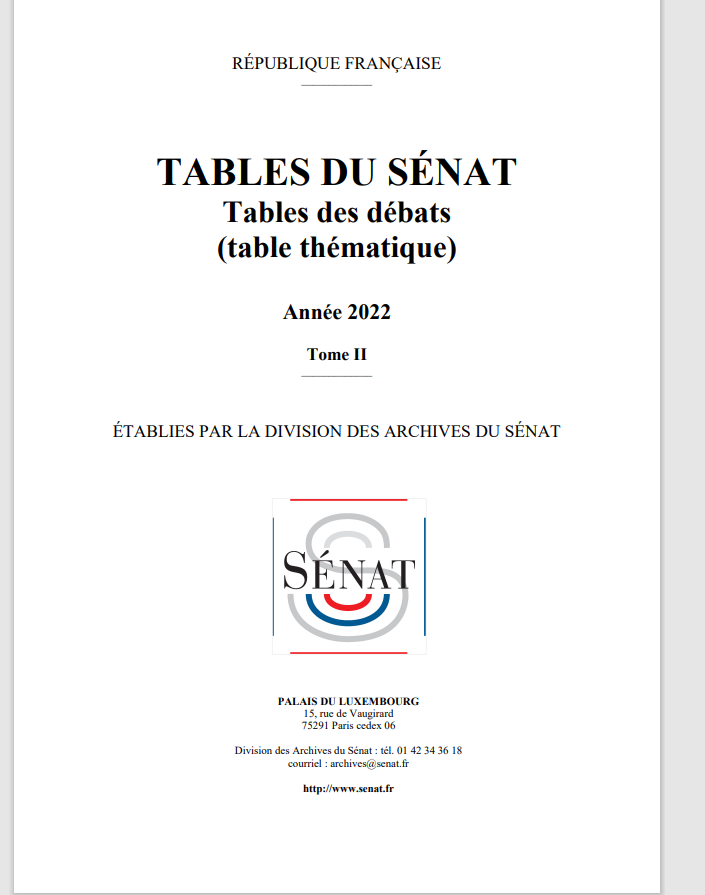
\includegraphics[width=0.6\textwidth]{images/tables thématiques .png}
    \caption{Capture d'écran des tables thématiques du Sénat\protect\footnote{Sources:https://www.senat.fr/les-tables-des-debats.html}}
\end{figure}

\subsubsubsection{Composition et activités des organes du Sénat (Tome III)}
Le troisième volume se concentre sur la composition et les activités des différents organes du Sénat. Il contient des listes détaillées des sénateurs, la composition des \gls{groupes_politiques}, du \gls{bureau_senat}, des \gls{commissions_permanentes} et \gls{commissions_temporaires}, ainsi que des \gls{delegations_structures}. Ce volume documente aussi les \gls{changements_organes}, la \gls{cour_justice_republique}, les \gls{organismes_extra_parlementaires}, les \gls{petitions}, et les \gls{rapports} remis au Parlement. Ce tome est basé sur les informations publiées dans le \textit{Journal officiel Lois et décrets}\footnote{Disponible sur: \url{https://www.legifrance.gouv.fr/jorf/jo}}, garantissant un suivi rigoureux et précis de l’activité parlementaire.
\begin{figure}
    \centering
    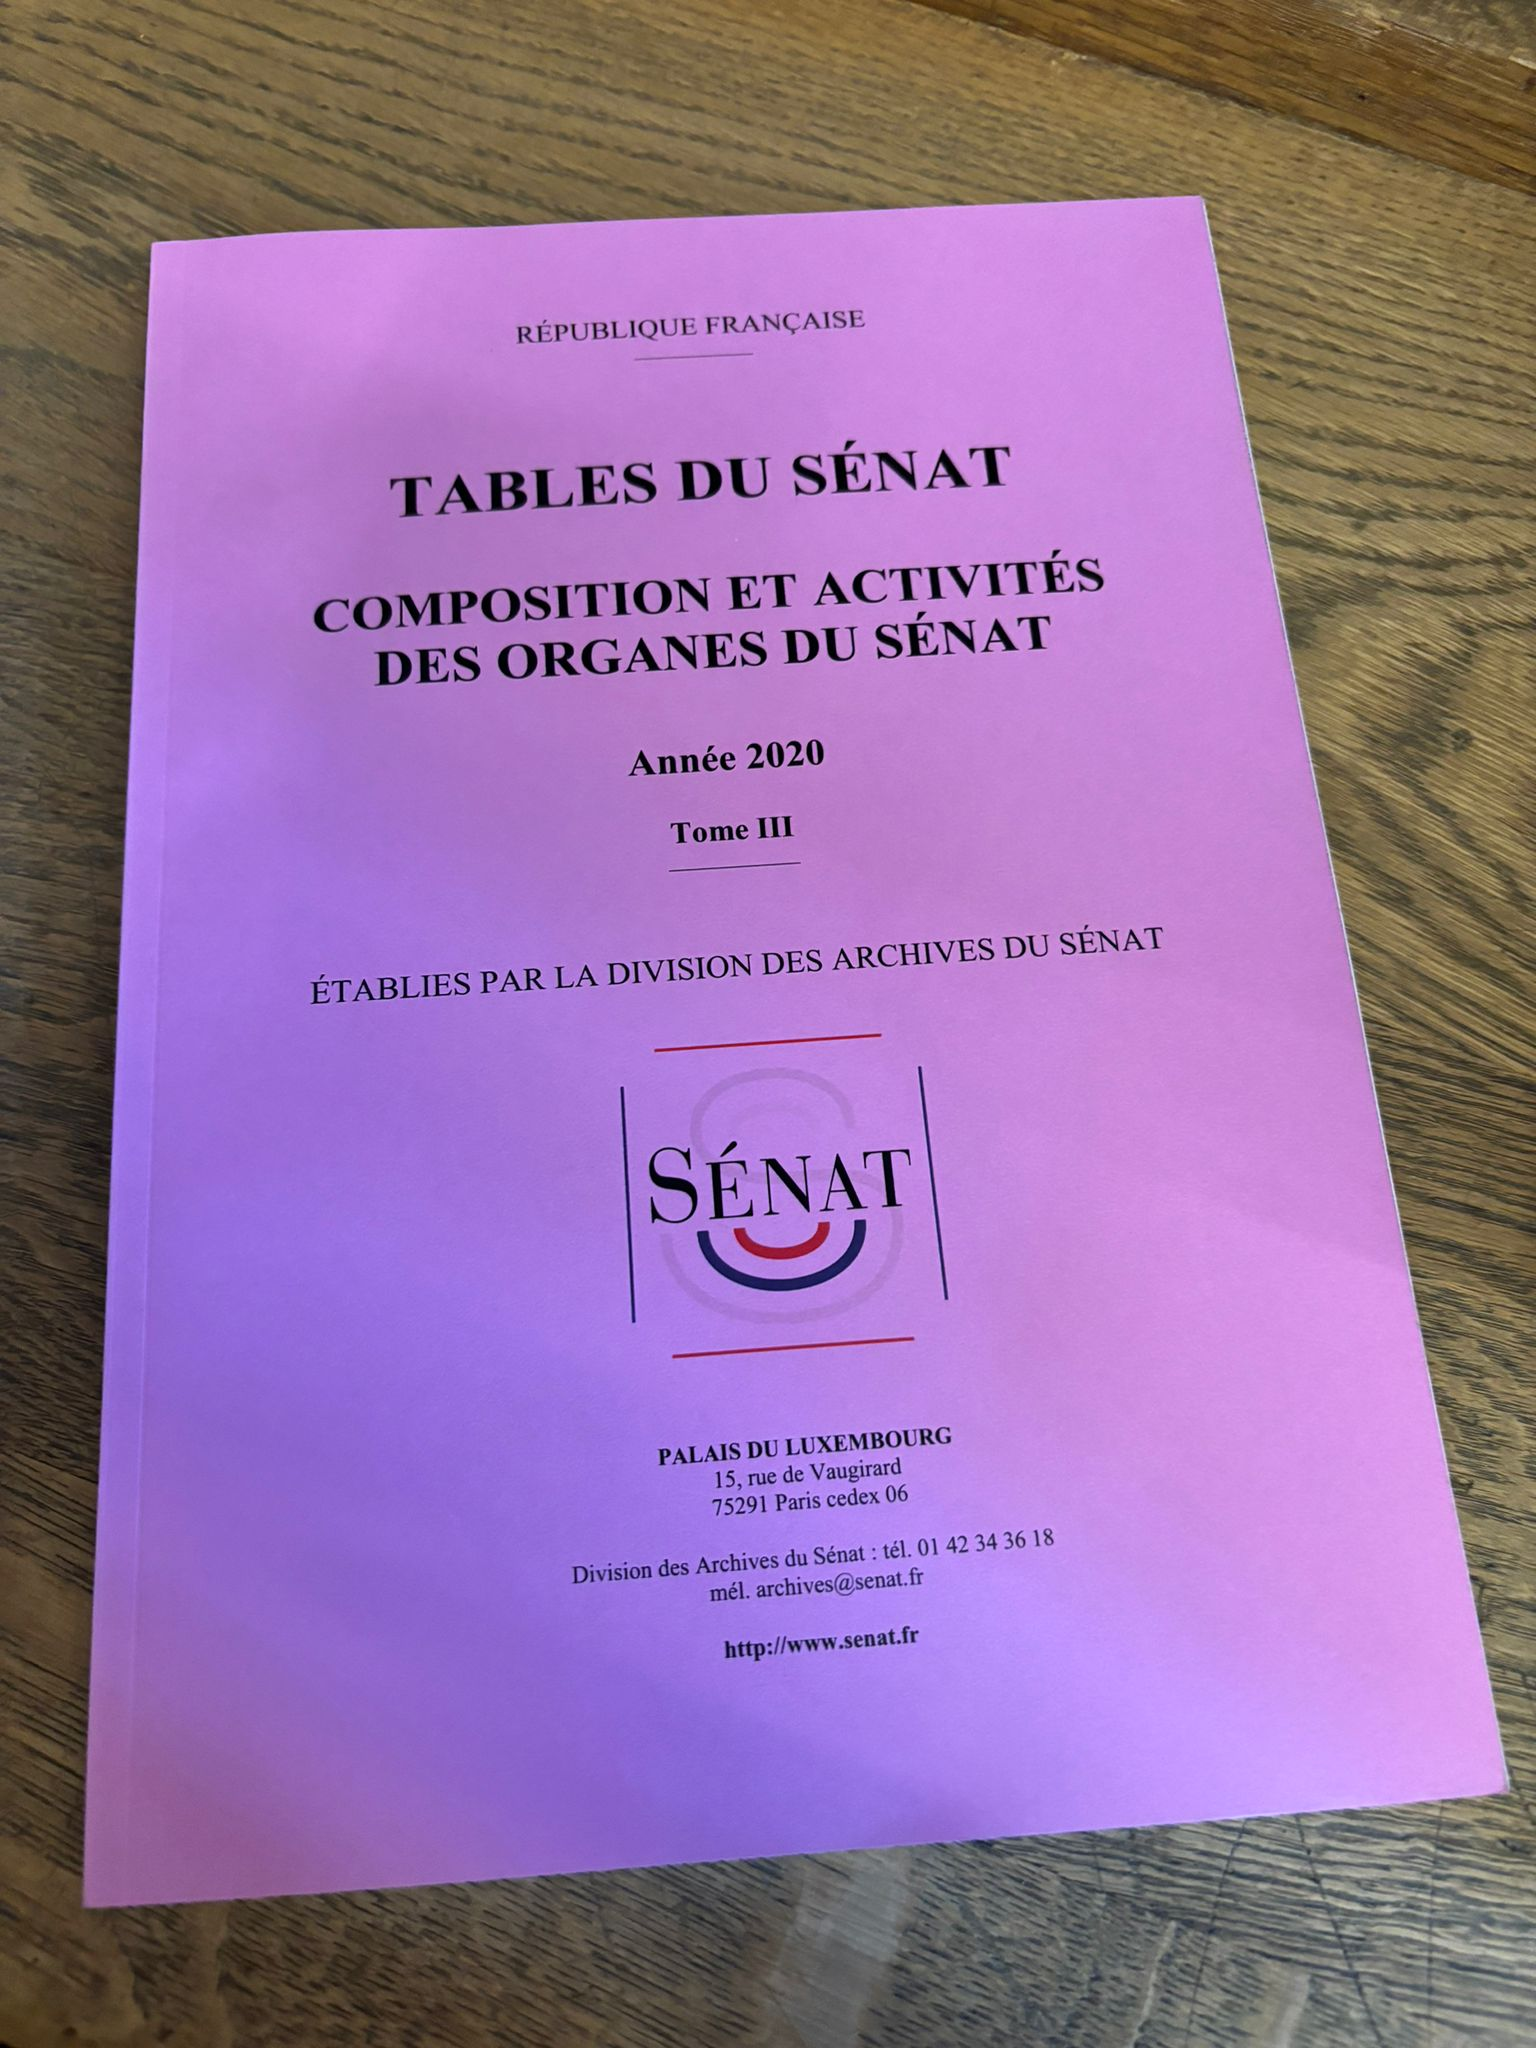
\includegraphics[width=0.5\linewidth]{images/tables3.jpg}
    \caption{Tables du Sénat- Tome III}
\end{figure}
Ces trois volumes, constituant les Tables des débats du Sénat, sont des ressources essentielles pour toute personne souhaitant suivre, analyser, ou étudier les travaux du Sénat français. Ces différentes tables constituent des outils indispensables pour la navigation et la recherche dans les archives parlementaires. Elles garantissent non seulement la transparence du processus législatif mais aussi la préservation de la mémoire institutionnelle du Sénat.

\section{L'importance des tables pour comprendre le fonctionnement de la séance publique}
\subsection{Intervenants de séance publique}

Les interventions en séance publique sont documentées de deux façons : par jour de séance et par texte de loi discuté. La présentation par jour de séance regroupe toutes les interventions de l’orateur pour une journée donnée, incluant à la fois les discussions sur les textes de loi et d'autres types de débats. En ce qui concerne la présentation par texte de loi, elle rassemble toutes les interventions de l’orateur relatives à un texte de loi spécifique. De plus, les projets de loi déposés par les ministres, ainsi que l’ensemble de leurs interventions en séance publique, sont également répertoriés dans la Table nominative.

L’équipe chargée des archives joue un rôle central dans ce processus en intervenant pour analyser les Journaux Officiels (JO). Grâce à leur travail minutieux, les données sont extraites, organisées et synthétisées afin d'être intégrées dans ces tables du Sénat. Leur intervention est essentielle pour garantir la précision et l’exhaustivité des informations présentées, permettant ainsi aux utilisateurs de naviguer facilement à travers les multiples débats et interventions. Cette contribution garantit que les tables du Sénat reflètent fidèlement les activités parlementaires et facilitent la recherche et l’analyse des débats par thème ou par sénateur.

\begin{figure}[H]
    \centering
    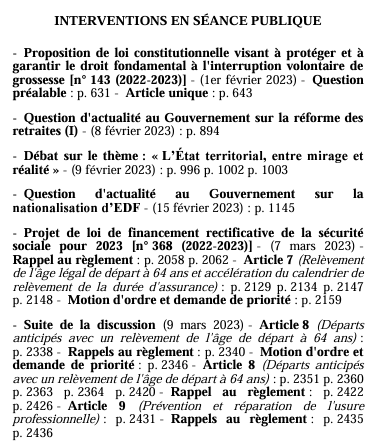
\includegraphics[width=0.5\linewidth]{images/Interventions Séances Publiques.png}
    \caption{Illustration d'intervention des Séances Publiques dans les Tables Nominatives\protect\footnote{source : \url{https://www.senat.fr/les-tables-des-debats.html}}}
\end{figure}

\subsection{Projet de loi et proposition de loi}

Un projet de loi est un texte législatif proposé par le gouvernement pour être examiné et adopté par le Parlement. Il émane généralement de l'exécutif et traduit la volonté politique du gouvernement de mettre en place une nouvelle législation ou de modifier des lois existantes. Les projets de loi sont souvent rédigés par les ministères concernés et soumis au Parlement après avoir été approuvés en Conseil des ministres. Une fois déposés, ils sont discutés en séance publique, où les sénateurs et les députés peuvent proposer des amendements avant de procéder au vote.

En revanche, une proposition de loi est un texte législatif proposé par un ou plusieurs parlementaires, sans l'intervention directe du gouvernement. Elle permet aux membres du Parlement d'initier des réformes législatives ou d'aborder des questions d'intérêt public qui ne sont pas nécessairement prioritaires pour l'exécutif. Comme les projets de loi, les propositions de loi sont examinées en séance publique, où elles peuvent être amendées et votées. Si elles sont adoptées par les deux chambres du Parlement, elles peuvent devenir des lois à part entière, au même titre que les projets de loi.

\section{Le processus de création des métadonnées de l’équipe d’archivistes}

\subsection{Équipe d'analyse et de bornage du JO aux archives}
Dans le processus d'élaboration des Tables du Sénat, l'analyse et le \gls{bornage} des JO sont fait par l'équipe de six personnes aux archives du Sénat.

\begin{figure}[H]
    \centering
    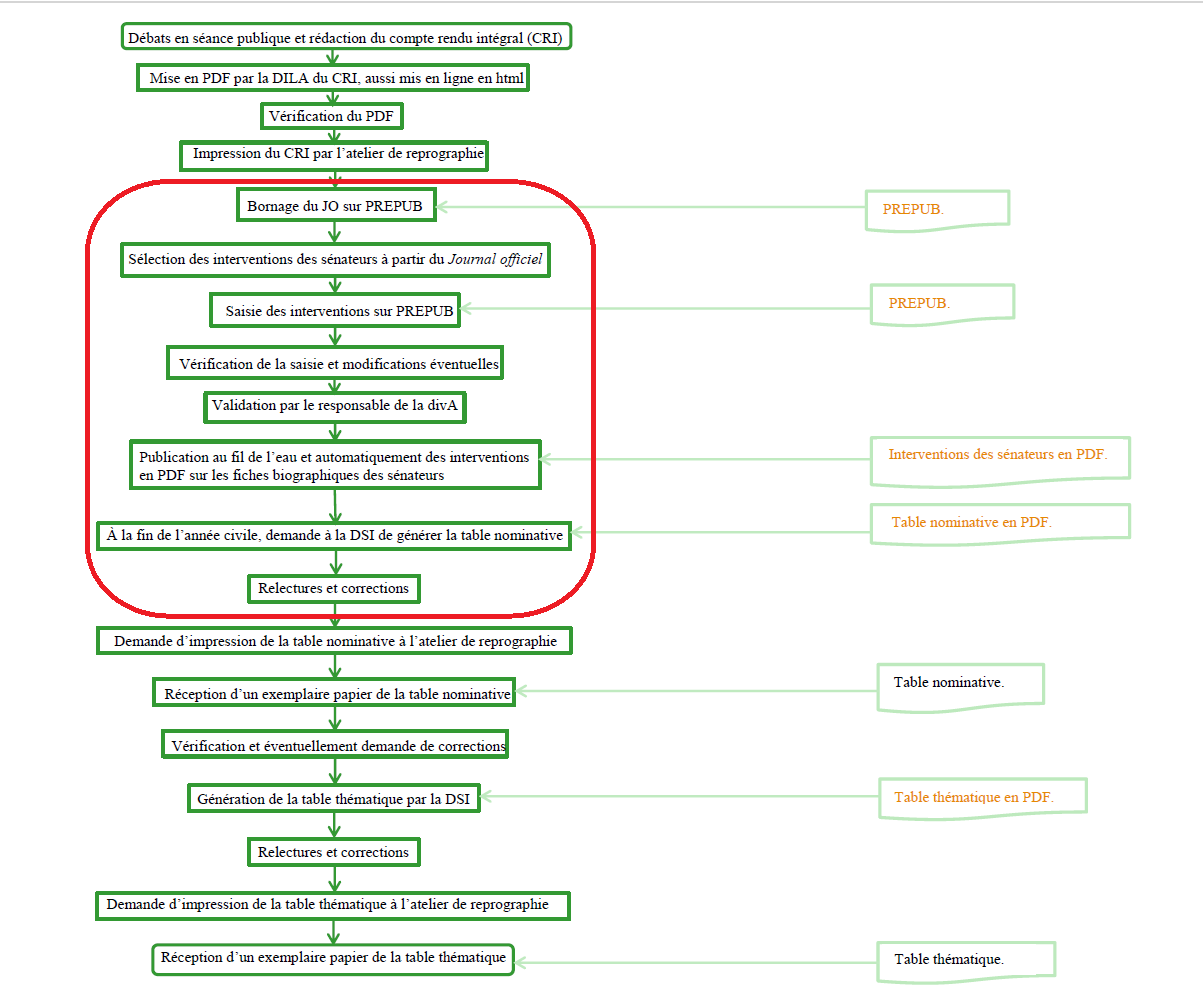
\includegraphics[width=1\textwidth]{images/Schéma de création les tables nominatives et thématiques.png}
    \caption{Schéma d'illustration des étapes de création d’instruments de recherche : les tables nominatives et thématiques \footcite{Lesdirectiondelabiblioetdesarchives}}
\end{figure}

Tout d'abord, les assistantes de gestion et de direction (ADG), Mme Line Zeppa, Mme Frédérique Pawloff et Mme Nathalie Palacios, s'occupent du traitement initial des Journaux officiels. Elles sont chargées de saisir les analyses de Madame Ghislaine Laumonerie concernant les projets de loi (PPL et PJL), ainsi que les interventions liées aux débats thématiques et aux questions diverses. En outre, elles effectuent les corrections demandées par M.Franck Pariguet et Mme Ghislaine Laumonerie. Cette étape constitue la base du processus de traitement des informations des JO.

Une fois le travail des ADG terminé, Mme Ghislaine Laumonerie, en tant qu’administratrice-adjointe, vérifie et valide les JO dans le système \gls{Prepub}. Elle est responsable de la sélection des interventions pertinentes à inclure dans les Tables du Sénat, ainsi que de la vérification finale des JO pour garantir leur exactitude avant de passer aux étapes suivantes. Elle gère également l’archivage et l’élimination des JO selon des délais fixés.

M.Franck Pariguet, en tant qu'assistant de gestion et de direction, poursuit en relisant les écrans de validation imprimés par les ADG. Il s’assure que la pagination est correcte, recherche les erreurs et garantit que toutes les données sont saisies de manière précise. Lorsqu'il détecte des erreurs ou des omissions, il demande aux ADG de procéder aux corrections nécessaires pour garantir l'intégrité des données.

Enfin, Mme Stéphanie Sanna, en tant qu’administratrice-adjointe, réalise la dernière vérification. Son rôle est de s'assurer que toutes les modifications additionnelles ont été correctement traitées. Une fois cette étape terminée, elle transmet la version papier du JO à Mme Ghislaine Laumonerie pour la validation finale dans le cadre du processus.

\subsection{Bornage et saisie des Journaux Officiels.}

\begin{figure}[H]
    \centering
    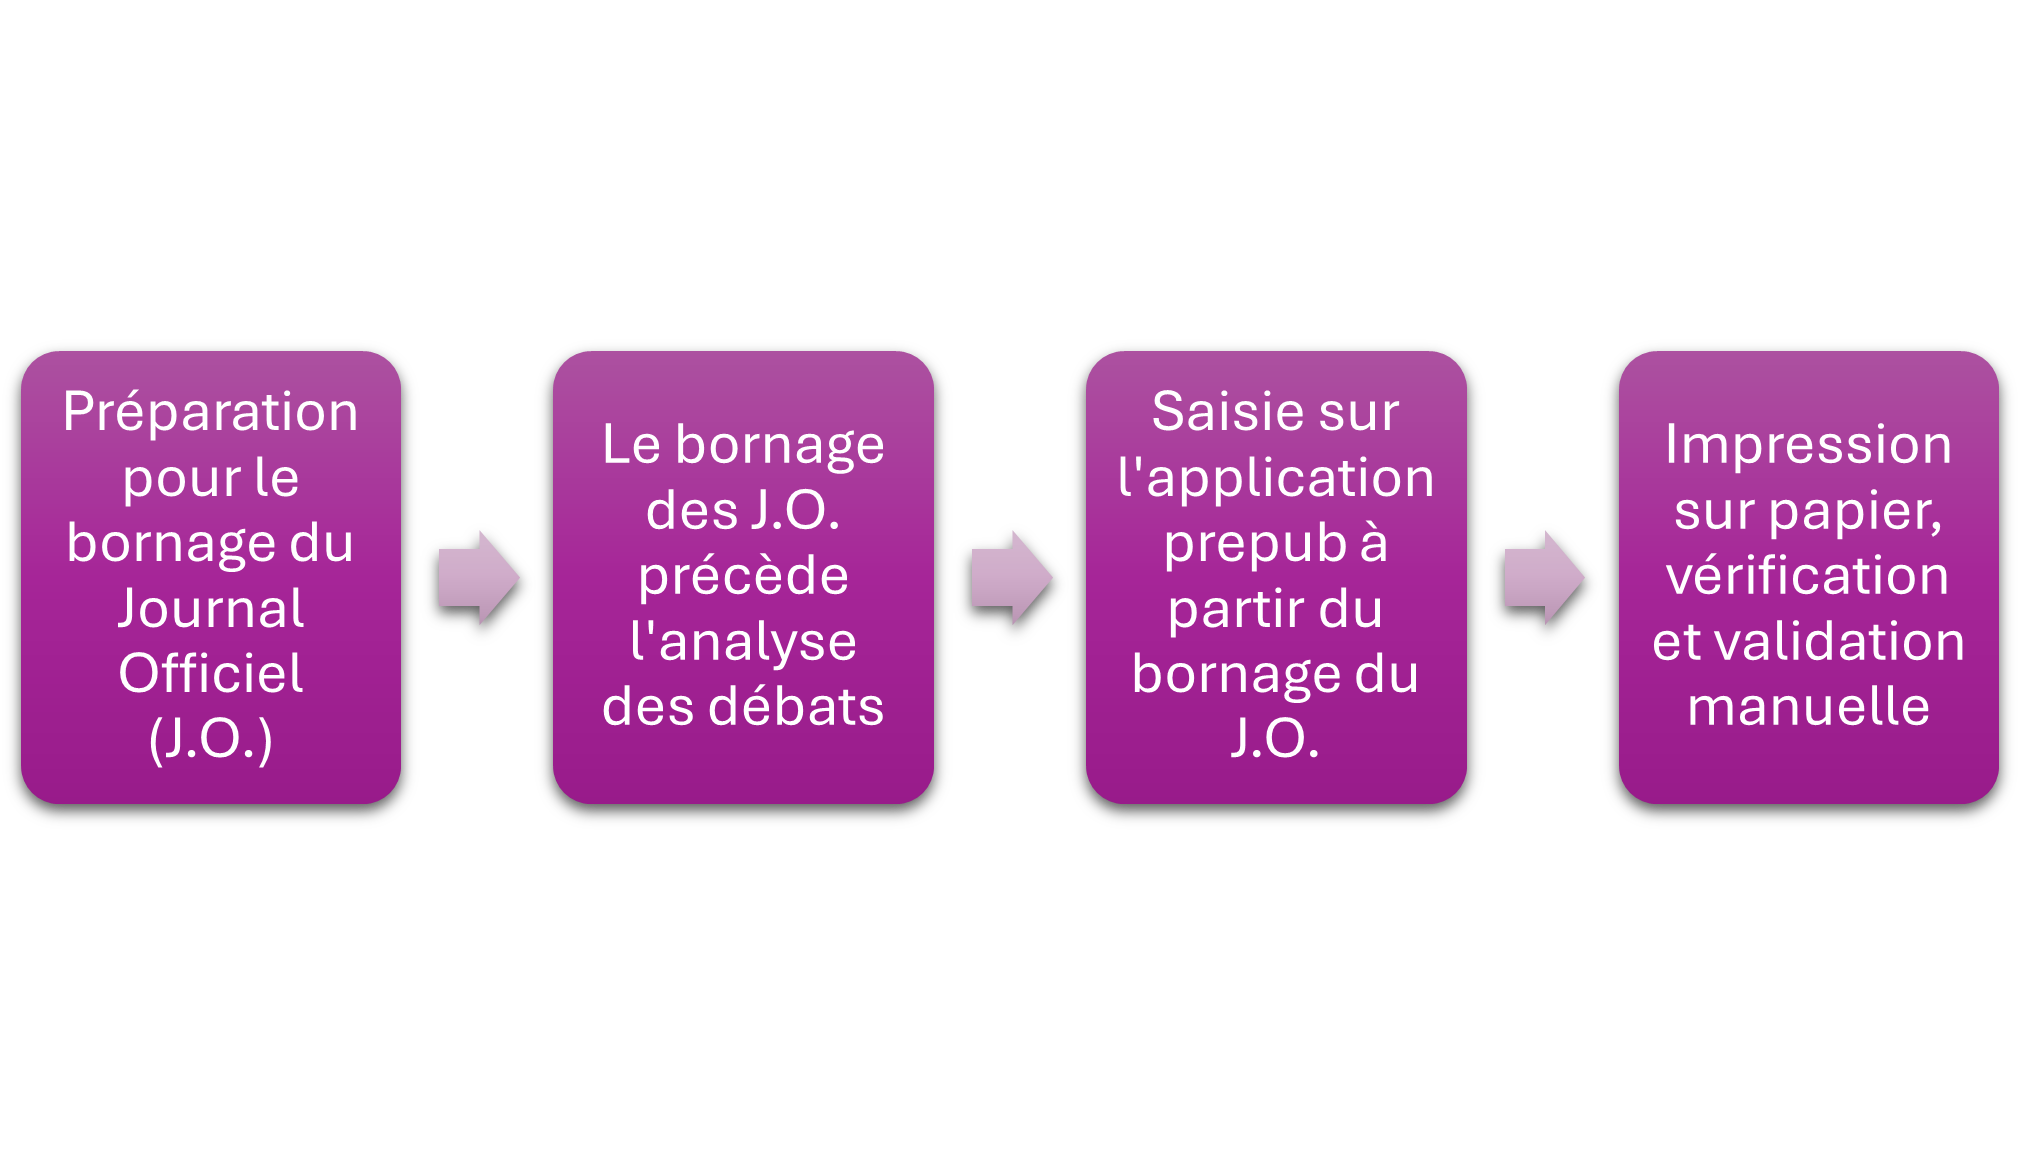
\includegraphics{images/Schéma Bornage Prepub.png}
    \caption{Schéma d'illustration des étapes du bornage dans Prepub}
\end{figure}

\paragraph{Préparation des JO papier}

Les JO papier sont annotés dès leur réception. La date de réception est inscrite sur la page de couverture, et des crayons de couleur sont utilisés pour identifier les sections importantes qui nécessitent une analyse approfondie.

\paragraph{Connexion à l'application Prepub}
%%%Prepub est un logiciel d'archivage interne au Sénat, il sert à la fois au moment du bornage, du choix des interventions et de leur saisir, ainsi qu'au moment de la validation finale du JO traité. 

L'utilisation de l'application \gls{Prepub} qui est un logiciel d'archivage interne au Sénat, il sert à la fois au moment du bornage, du choix des interventions et de leur saisir, ainsi qu'au moment de la validation finale du JO traité, suit la préparation initiale du JO papier. Cette application, spécifique à la division des Archives du Sénat, permet le bornage numérique des Journaux Officiels, facilitant la navigation et l'utilisation des menus déroulants pour marquer les sections préalablement soulignées.

\paragraph{Le bornage proprement dit};

Le bornage implique plusieurs sous-étapes :

\begin{itemize}
    \item \textbf{Bornage des Textes de Lois}: L'application Prepub est utilisée pour naviguer à travers le sommaire et délimiter les textes de loi, marquant les débuts et les fins des discussions.

\begin{figure}[H]
    \centering
    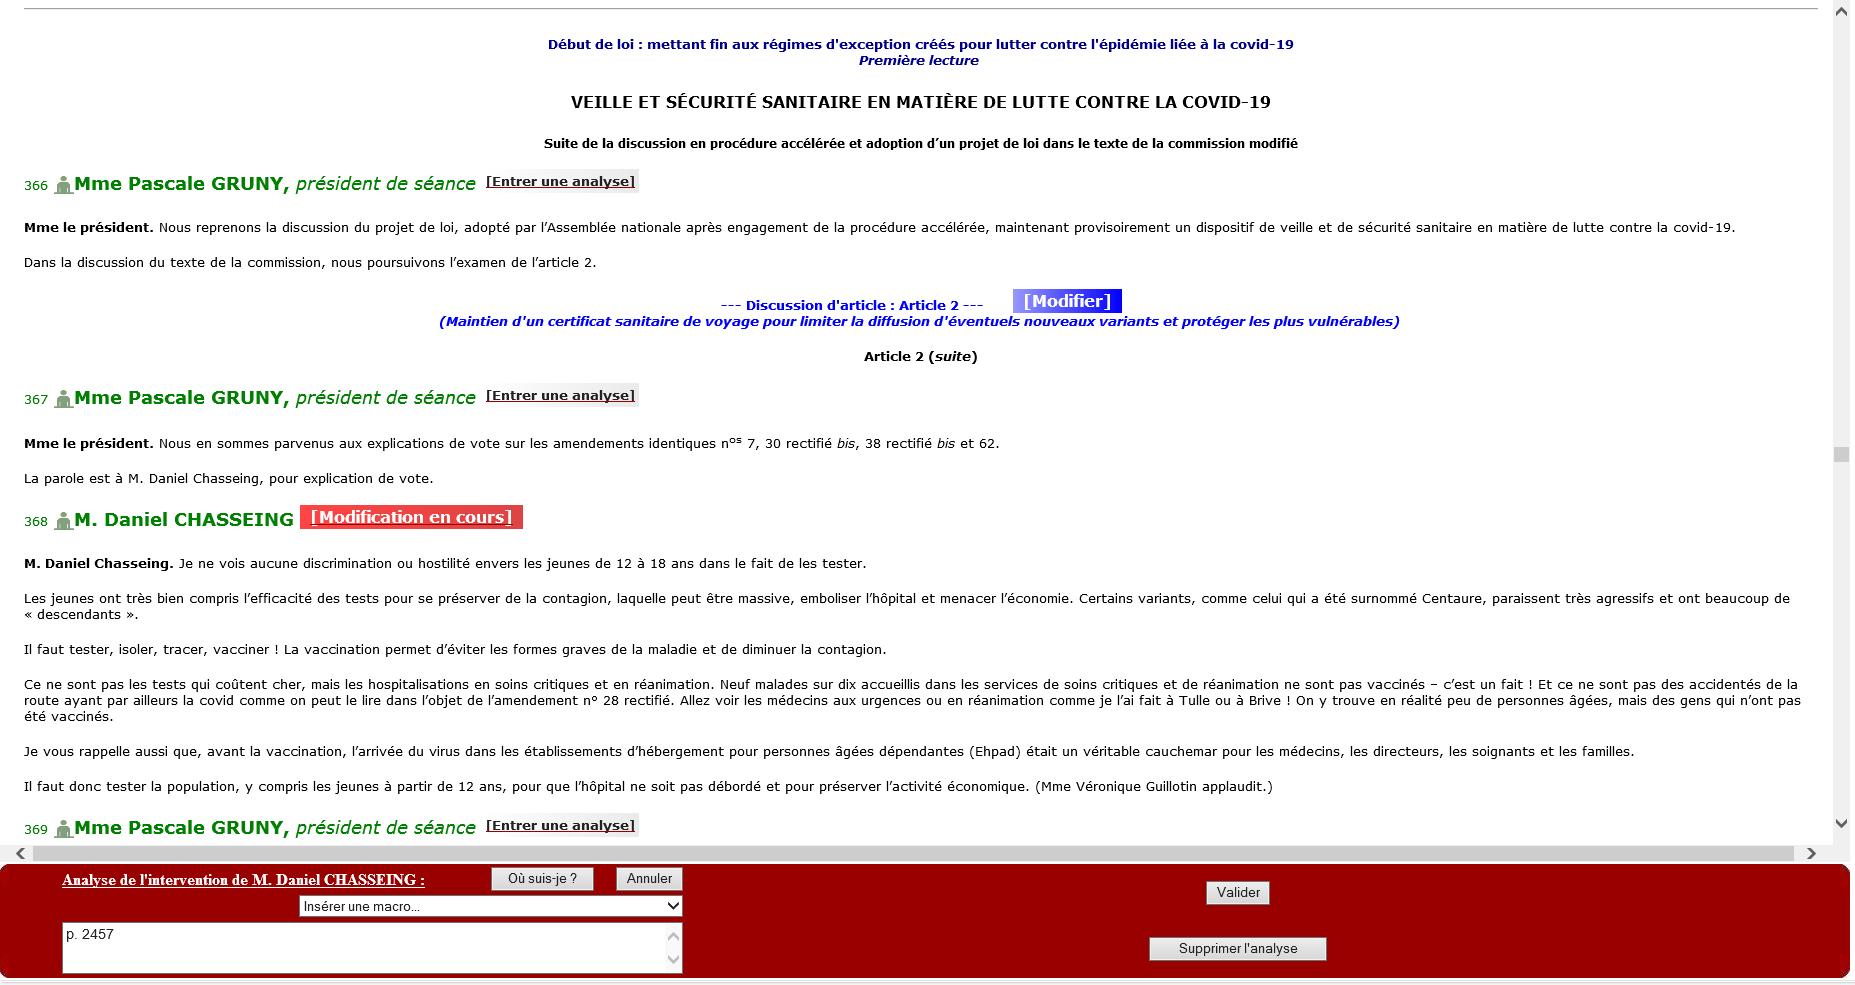
\includegraphics[width=1\linewidth]{images/article.png}
    \caption{Capture d'écran d'application de Prepub}
\end{figure}
    
    \item \textbf{Bornage de textes législatifs hors lois}: Les interventions non liées directement aux textes de loi, comme les allocutions, sont également bornées en utilisant des subdivisions appropriées dans l'application.
\end{itemize}

\paragraph{Vérification et impression}

Une fois le bornage terminé, une vérification est effectuée pour valider l'exactitude des informations. Le processus se conclut par l'impression du bornage pour une relecture, ce qui comprend la date du bornage et les initiales de la personne ayant réalisé le travail, assurant ainsi une traçabilité et une validation finale avant l'enregistrement officiel des données. 

Ces étapes détaillées illustrent l'engagement et la rigueur de l'équipe d'archivistes dans la gestion des métadonnées du Journal Officiel, garantissant une documentation précise et accessible des activités parlementaires.

\subsection{Processus actuel de collecte et de gestion des métadonnées}

L'équipe d'archivage travaille en étroite collaboration avec la Direction du Compte Rendu (DCR) et la Direction des Systèmes d'Information (DSI) pour optimiser la gestion des métadonnées. Les étapes clés de ce processus comprennent les processus suivants:

\begin{figure}[H]
    \centering
    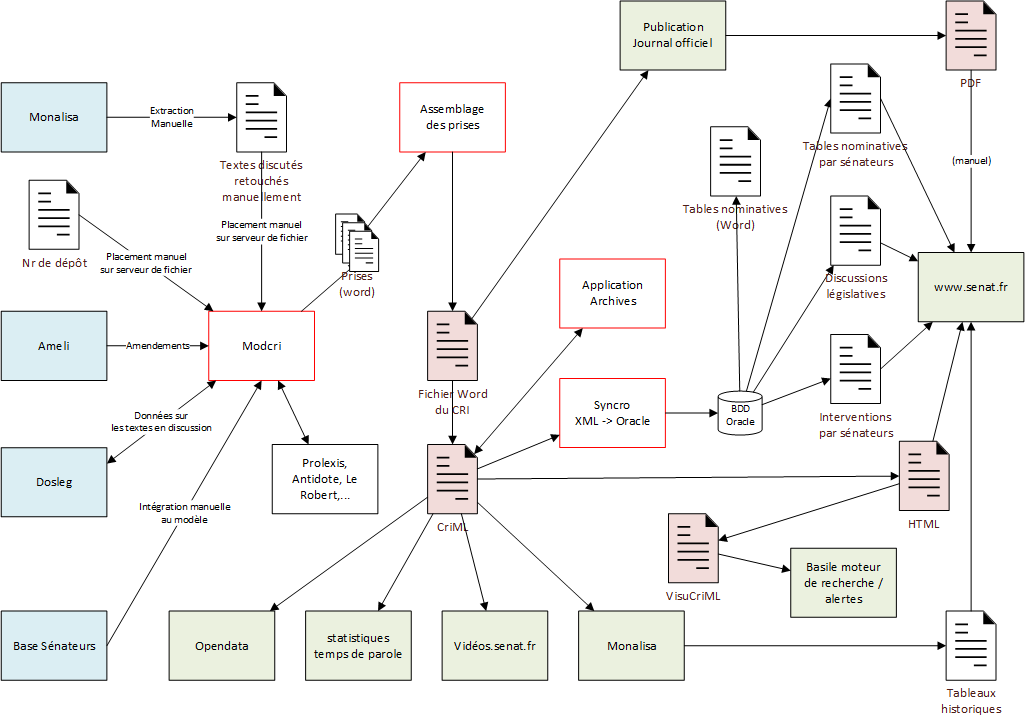
\includegraphics[width=1\linewidth]{images/cri.png}
    \caption{Schéma SI lien avec CRI, fournit par les archivistes du Sénat}
\end{figure}


\subsubsection{Initialisation et Conversion des Documents}

Les comptes rendus sont d'abord rédigés en format WORD (.DOCX) par la DCR avant d'être convertis en format .DOC pour transmission à la \gls{DILA}, une étape automatisée pour assurer l'uniformité et la compatibilité des fichiers. Ces documents sont ensuite transformés de .\gls{XML} en .\gls{HTML} pour une publication en ligne, suivie d'une conversion finale en format \gls{PDF} validée par la \gls{DILA} en vue d’une diffusion plus large, y compris sur Légifrance.\footcite{VadeMecum}

\subsubsection{Gestion Documentaire et Vérifications}

La DCR, en plus des conversions de format, intègre des macros dans le modèle WORD utilisées pour insérer automatiquement des phrases types fréquemment utilisées, facilitant ainsi la standardisation des procédures telles que les prises de parole et les mises aux voix. Des vérifications supplémentaires sont effectuées par des membres de la DCR, comme Guillaume JANDOT, pour s'assurer de la précision des comptes rendus avant leur publication dans l’application Prepub.\footcite{VadeMecum}

\subsubsection{Publication et Accès aux Données}

- Les fichiers finalisés destinés à l'Open Data, c'est à dire à la publication "ouverte" sur le site du Sénat, sont exportés depuis \gls{Prepub} en format .\gls{XML}, avec leurs métadonnées associées, vers les serveurs du site senat.fr\footnote{Fichiers .\gls{XML} et .\gls{SQL} accessibles ici : https://data.senat.fr/la-base-comptes-rendus/} permettant une accessibilité et une réutilisation optimales des données pour tous. 
- Les Tables des séances, tout comme la Table nominative, sont quant à elles générées à partir de l'ensemble des informations contenus dans ces fichiers source .\gls{XML}/.\gls{SQL} et rationalisent les entrées listées dans ces bases de données grâce au logiciel \gls{Prepub} afin de publier son contenu sous format .\gls{PDF} dans le JO électronique.

\subsubsection{Assemblage et Publication des Fichiers}

Chaque compte rendu, composé initialement de plusieurs fichiers .WORD rédigés par différents auteurs, est assemblé pour former un document \gls{XML} unique par séance. En collaboration avec la DSI, des schémas explicatifs du système informatique lié au CRI ont été élaborés pour illustrer le flux de données et leur traitement.

Ces étapes illustrent un processus complexe et intégré de gestion des métadonnées qui non seulement permet un archivage précis des activités parlementaires mais assure également une transparence et une accessibilité accrues pour le public et les chercheurs. Les défis liés à ce processus, notamment la gestion manuelle et la complexité des formats, nécessitent une vigilance continue pour maintenir l'intégrité et la précision des archives.
\section{Analyse des limitations et des défis du processus manuel}

Le processus manuel de gestion des métadonnées du \gls{JO} par l'équipe d'archivistes présente plusieurs défis significatifs liés à la consommation de ressources humaines et au temps nécessaire pour assurer la précision des archives :

\subsubsection{Intensité de la main-d'œuvre}

La gestion manuelle des métadonnées du \gls{JO} nécessite l'implication d'une équipe de six personnes, qui doivent lire et relire chaque édition pour en assurer l'exactitude. Cette approche est extrêmement exigeante en termes de ressources humaines, chaque membre de l'équipe devant examiner minutieusement les documents pour identifier et corriger les erreurs potentielles. Cette intensité de la main-d'œuvre rend le processus non seulement coûteux mais aussi sujet à des risques d'erreur accrus du fait de la fatigue et des erreurs humaines.

\subsubsection{Consommation excessive de temps}

Le processus requiert que chaque \gls{JO} soit passé en revue plusieurs fois pour s'assurer que toutes les métadonnées sont correctement bornées et enregistrées. Cette révision multiple est chronophage, retardant potentiellement la disponibilité des informations pour les utilisateurs finaux et impactant l'efficacité globale de l'archivage. La nécessité de multiples lectures et de vérifications augmente le risque d'erreurs humaines dans le bornage et la saisie des métadonnées. Chaque erreur nécessite des révisions et des corrections supplémentaires, augmentant encore le temps consacré à chaque \gls{JO} et exacerbant la charge de travail de l'équipe.

\subsubsection{Dépendance à la précision humaine}

La dépendance du processus à la précision humaine dans la lecture et la saisie des données peut entraîner des incohérences et des lacunes dans les archives. Cette situation est particulièrement problématique dans un contexte où les erreurs peuvent compromettre l'intégrité des données historiques et législatives, essentielles pour les recherches et les références futures.

\subsubsection{Une mise à l’échelle limitée}

La mise à l’échelle du processus est limitée par la capacité humaine à gérer un volume toujours croissant de données. Sans possibilité d'augmenter de manière flexible le nombre de membres de l'équipe ou d'intégrer des solutions techniques avancées, il est difficile de répondre efficacement aux besoins changeants de gestion des archives.

Ces limitations mettent en évidence la nécessité d'adopter des méthodes plus automatisées et moins dépendantes de l'intervention humaine intensive. L'automatisation pourrait réduire le nombre de lectures nécessaires, diminuer le risque d'erreurs, et améliorer la rapidité de traitement des \textit{Journaux Officiels}, tout en conservant les ressources précieuses de l'équipe d'archivistes.